\begin{graphicspathcontext}{{./chapters/sarl/imgs/},{./chapters/sarl/imgs/auto/},\old}

\begin{frame}{Why a New Agent Language?}
	\begin{block}{Observation}
		Modern software systems are increasingly \Emph{distributed}, \Emph{concurrent}, \Emph{adaptive}, and \Emph{open}
	\end{block}
	\vspace{.5em}
	\Emph{Limitations of existing approaches:}
	\begin{description}
	\item[Object-Oriented Programming] no built-in autonomy or reactivity model
	\item[Existing AOP Languages] either too specific or poorly integrated with
	  mainstream JVM ecosystems (or with other main stream languages)
	\end{description}
	\vspace{.5em}
	\begin{alertblock}{Goal of SARL}
		Provide a \Emph{general-purpose}, agent programming language that combines \emph{expressiveness}, \emph{modularity}, and \emph{platform independence}
	\end{alertblock}
\end{frame}

\begin{frame}{What is SARL?}
	\begin{columns}[T]
		\begin{column}{.8\linewidth}
			\begin{itemize}
			\item A \Emph{statically-typed, JVM-compiled} language
			\item Built on top of the \Emph{Xtext/Xbase} framework
			\item Full \Emph{interoperability} with Java and other JVM languages
			\item Equipped with an \Emph{Eclipse-based IDE}
			\item Runs on the \Emph{Janus SRE} (SARL Runtime Environment)
			\item First release: 2014 --- actively maintained (v\sarlversion, \sarlreleaseyear)
			\item Open-source --- Apache License 2.0
			\end{itemize}
		\end{column}
		\begin{column}{.2\linewidth}
			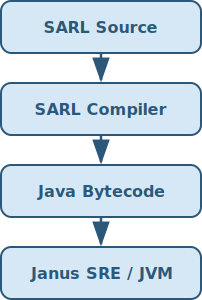
\includegraphics{sarl_pipeline}
		\end{column}
	\end{columns}
\end{frame}

\begin{frame}{{Design Principles} of SARL}
	\begin{enumerate}
	\item \Emph{Separation of Concerns} \\
	{\footnotesize What an agent \emph{can do} (Capacity) is separate from \emph{how} it does it (Skill)}
	\vspace{.3em}
	\item \Emph{Event-Driven Interaction by Default} \\
	{\footnotesize Agents communicate by default through typed, asynchronous events}
	\vspace{.3em}
	\item \Emph{Holonic / Hierarchical Organisation} \\
	{\footnotesize Agents are organized in Contexts; an agent can be a member of multiple contexts simultaneously}
	\vspace{.3em}
	\item \Emph{Openness \& Extensibility} \\
	{\footnotesize New capacities, skills and spaces can be plugged in at runtime}
	\vspace{.3em}
	\item \Emph{Platform Independence} \\
	{\footnotesize SARL code is independent of the underlying SRE; the runtime behaviour is injected via built-in capacities.}
	\end{enumerate}
\end{frame}

\figureslide{SARL Architecture}{sarl_architecture}

\begin{frame}{Holonic Architecture}
	\begin{columns}
		\begin{column}{.7\linewidth}
			SARL supports \Emph{holonic multi-agent systems}:
			\begin{itemize}
			\item Every agent \emph{defines} its own inner context
			\item Sub-agents can be spawned \emph{inside} this inner context
			\item The parent agent acts as a \Emph{super-agent} (holon)
			\item Each agent is both:
				\begin{itemize}
				\item A \emph{member} of its parent's context
				\item The \emph{super-agent} of its inner context
				\end{itemize}
			\item Enables natural hierarchical decomposition of complex systems
			\end{itemize}
		\end{column}
		\begin{column}{.3\linewidth}
			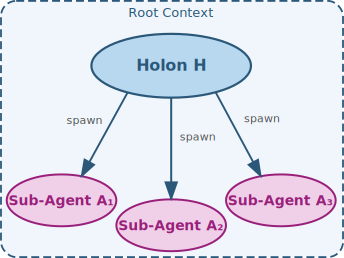
\includegraphics{sarl_holonic}
		\end{column}
	\end{columns}
\end{frame}

\begin{frame}[t]{Summary}
	\begin{block}{SARL in one sentence}
	SARL is a \Emph{general-purpose, JVM-compiled agent programming language} that provides first-class constructs for \emph{agents}, \emph{behaviors}, \emph{capacities}, \emph{skills}, \emph{events}, \emph{spaces}, and \emph{contexts} — enabling expressive, modular, and platform-independent development of multi-agent systems
	\end{block}
	\vspace{.25cm}
	\begin{columns}
		\begin{column}[t]{.5\linewidth}
			\Emph{Key strengths}
			\begin{compactitemize}
			\item Holonic architecture natively supported
			\item Clean separation of capacity and skill
			\item Reactive model via guarded behavior units
			\item Full Java interoperability
			\item Rich IDE and toolchain
			\end{compactitemize}
		\end{column}
		\begin{column}[t]{.5\linewidth}
			\Emph{Resources}
			\begin{compactitemize}
			\item Website: \texttt{http://www.sarl.io}
			\item Source:  \texttt{github.com/sarl/sarl}
			\item License: Apache 2.0
			\end{compactitemize}
		\end{column}
	\end{columns}
\end{frame}

\end{graphicspathcontext}

\endinput

